\section{Durchführung}
\label{sec:Durchführung}

\subsection{Erzeugung niederenergetischer Neutronen}
    Zunächst werden Neutronen durch den Beschuss von $^9Be$-Kernen mit $\alpha$-Teilchen erzeugt. Da
    wie in Kapitel \label{sec:Neutronen} langsame Neutronen einen besonders hohen Wirkungsquerschnitt
    aufweisen, werden sie in Paraffin abgebremst. Die verwendete Apparatur ist in Grafik \ref{fig:machdeinearbeit} gezeigt. 
    \begin{figure}[H]
        \centering
        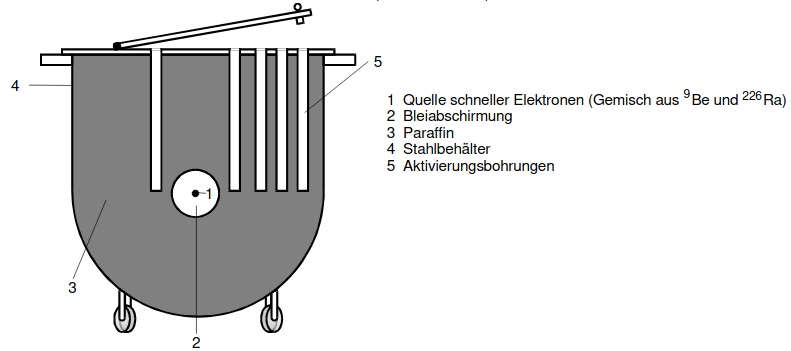
\includegraphics[width=\textwidth]{Neurosen.png}
        \caption{Aufbau zur Aktivierung der Proben.}
        \label{fig:machdeinearbeit}
    \end{figure}
    Die zylinderförmigen Proben werde also in die Aktivierungsbohrungen eingeführt, um die Materialien 
    anzuregen.
\subsection{Untersuchung des Zerfalls}
    Die angeregten Proben werden nun wiederum mit der in \ref{fig:lailai} dargestellten Apparatur untersucht.
    \begin{figure}[H]
        \centering
        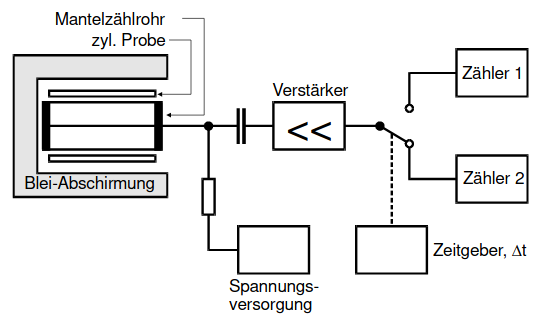
\includegraphics[width=\textwidth]{Aufbau.png}
        \caption{Versuchsaufbau.}
        \label{fig:lailai}
    \end{figure}
    Um die Umgebungsradioaktivität möglichst gering zu halten wird der Versuchsaufbau nach 
    außen hin durch Blei abgeschirmt. Trotzdem exestiert bereits ohne Probe ein Nulleffekt $N_u$, 
    der insbesondere bei kleinen Zählraten vor der eigentlichen Messung bestimmt werden muss. 
    Bei einem Ausschlag des Geiger-Müller-Zählrohrs wird 
    am Verstärkerausgang ein elektrischer Impuls generiert. Dieser wird an ein elektronisches
    Zählwerk mit zwei Anzeigevorrichtungen weitergeleitet, sodass ununterbrochen gemessen 
    werden kann. 